\section{Experiment}
\label{ch3-sec:experiments}

\newcommand{\dgef}{$DGE_{flow}$\xspace}
\newcommand{\dges}{$DGE_{spatial}$\xspace}
\newcommand{\hdge}{$HDGE$\xspace}

In this section, we first describe datasets and experiment settings. Then we evaluate the effectiveness and efficiency of proposed embedding method with several prediction tasks. Finally, we interpret the semantic meaning of the learned embedding with both quantitative analysis and case study.


\subsection{Settings}

\subsubsection{Data description.} We study the urban dynamics at community area (CA) level. A community area is a predefined administrative area in the city of Chicago. The geographic boundary information is available through US census survey~\cite{data-census}. The following urban data are collected and used in our evaluation.

\textbf{Demographics data} at community area level is made public by the US census bureau~\cite{data-census}. The demographic features mainly cover the following aspects of a community area: total population, population density, poverty, residential stability, and ethnic diversity.

\textbf{Point-Of-Interest (POI) data} is obtained through Foursquare API~\cite{data-poi}. It contains more than $112,000$ POI records for Chicago. Each POI record provides venue name, category, number of check-ins, and number of unique visitors. We use the POI category distribution information of each region to measure the region functions. There are 10 major POI categories including arts \& entertainment, education, event, food, nightlife, outdoor \& recreation, professional, residence, shops and travel.

\textbf{Taxi data}~\cite{data-taxi} in Chicago from 2013 to 2015 are used to construct the mobility flow graph. There are over $86$ million taxi trips recorded over the three years, which is roughly $2.4$ million trips per month. For each trip, we have the following information available: pick-up and drop-off dates and locations. Due to privacy concern, in this dataset, all timestamps are rounded to closest 15 minute marks, and all locations are mapped to the center of census tracts.

\textbf{Crime data} is publicly available on Chicago Data Portal~\cite{data-crime}, which contains more than 5 million crime incidents from 2001 to current day. The incident date, location, and primary type of each crime incident are recorded.

\textbf{House price data} is obtained from Zillow real estate website~\cite{data-houseprice}. We collect the sale price, floor size, latitude, and longitude information for over $45,000$ real estates that were sold within 2 years in the city of Chicago.
\smallskip

In order to evaluate and interpret our embedding results, we predict the following three target variables for each community area.
\begin{itemize}[leftmargin=*]
\item Crime rate, which is crime incidents count per 10,000 population.
\item Average personal income in dollar.
\item Average house price with a unit of dollar per square foot.
\end{itemize}


\subsubsection{Methods for comparison}

For each prediction task, we follow the generalized regression framework in Equation~(\ref{eq:nbr}). We use the state-of-the-art method in \cite{wang2016crime} as a base model, which does not employ the embedding technique to calculate relevances. Since the base model directly employs the traffic volume and inverse spatial distance as relevance measure, we denote it $RAW$ in the rest of experiments.

We name our embedding method as \textbf{heterogeneous dynamic graph embedding (\hdge)}. This proposed dynamic embedding technique also applies to single flow graph or spatial graph, which are called \dgef and \dges respectively. 
We set the embedding dimension as $8$ for all methods. We compare \hdge with two alternative embedding methods. First, we introduce a straightforward baseline approach for flow graph modeling, called \emph{slotted graph}. Similar to flow graph, the slotted graph also accounts for the temporal dynamics. However, the slotted graph models the mobility flow for each time slot independently.
\begin{itemize}[leftmargin=*]
\item \textbf{Matrix factorization ($MF$)} is a conventional method for dimension reduction. In order to get dynamic vector representations, the matrix factorization method is used to decompose the adjacency matrices of slotted graphs.
\item \textbf{LINE}~\cite{tang2015line} is a graph embedding method that learns embedding on a weighted graph to encode both first and second order proximity. Applying LINE on the slotted flow graph also leads to an alternative temporal embedding.
\end{itemize}


\subsubsection{Evaluation metrics}

The dynamic embedding method learns different embeddings for different time slot. Within each time slot, we use leaned embeddings to calculate the relevance measures and evaluate the regression model with leave one out setting. The model performance is evaluated by mean relative error and mean absolute error:
\begin{equation*}
MRE = \frac{1}{T} \sum_{t=1}^T \frac{\sum_i^n |y_{it} - \hat{y_{it}}|}{\sum_i^n y_{it}} \quad
MAE = \frac{1}{T} \sum_{t=1}^T \sum_i^n |y_{it} - \hat{y_{it}}|,
\end{equation*} 
where $y_{it}$ is the ground truth value for target variable of region $i$ at time slot $t$, and $\hat{y_{it}}$ is the estimate.

It is worthy mentioning that among all three target variables only crime rate presents daily periodicity. For average personal income and real estate price, the value of the same region does not change within one day, i.e. $\forall t \in \mathcal{T},$ $y_{it} = y_i$.









\subsection{Evaluations}

\subsubsection{Feature Selection}

For each predication task, we have four types of features available, which are demographic features (D), POI features (P), geographical feature (G), and taxi flow feature (T). In this section, we aim to identify the best feature combinations for each prediction task. We use the base model $RAW$ for this purpose.



\begin{table}[h]
\centering
\caption{Crime rate prediction with $RAW$ from 2013 to 2015. The MAE unit is crime count per 10,000 population.}
\label{exp:crime}
\begin{tabular}{|l|r|r|r|r|r|r|}
\hline
Year & \multicolumn{2}{c|}{2013} & \multicolumn{2}{c|}{2014} &  \multicolumn{2}{c|}{2015} \\ \hline
Features$^1$ & MAE & MRE & MAE & MRE & MAE & MRE \\ \hline
D+P	& 15.03	& 0.318	& 13.26 & 0.317	& 7.31	& 0.335 \\ \hline
D+P+G &	15.54	& 0.329	& 13.75	& 0.326	 & 7.46	& 0.337\\ \hline
\rowcolor{Gray}
D+P+T &	14.52	&0.308	&12.79	&0.307	&7.15	&0.322 \\ \hline
D+P+G+T &	14.92	&0.316	&13.15	&0.316	&7.35	&0.332\\ \hline
\end{tabular}

\footnotesize{$^1$ D -- demographic features, G -- geographical influence, P -- POI features, T -- taxi flow feature.\\}
\end{table}

The crime rate prediction results of $RAW$ method with different feature combinations are shown in Table~\ref{exp:crime}. We only show the prediction results from year 2013 to 2015, because only in those years we have both taxi flow data and crime incident data. From Table~\ref{exp:crime}, we observe that the best crime rate prediction is achieved by using only three types of features, i.e. demographics, POI, and taxi flow. Adding geographic features does not improve the prediction accuracy. This observation is actually consistent with previous work \cite{wang2016crime}. 


\begin{table}[h]
\centering
\caption{Average personal income and house price prediction with $RAW$. The MAE unit of personal income is dollar. The MAE unit of house price is dollar per square foot.}
\label{exp:other}
\begin{tabular}{|l|r|r|r|r|}
\hline
Data & \multicolumn{2}{c|}{Income} & \multicolumn{2}{c|}{House Price}  \\ \hline
Features & MAE & MRE & MAE & MRE  \\ \hline
D+P	& 15304 &	0.253 & 39.87 & 0.233 \\ \hline
D+P+G &	16905 &	0.279 & 41.40 & 0.242 \\ \hline
D+P+T &	15433 &	0.255 & \cellcolor{Gray} 39.28 & \cellcolor{Gray} 0.229  \\ \hline
D+P+G+T & \cellcolor{Gray}	15127 & \cellcolor{Gray} 0.250 & 40.728 & 0.238 \\ \hline
\end{tabular}
\end{table}


The average personal income and house price prediction results of $RAW$ are shown in Figure~\ref{exp:other}. When making income prediction, we eliminate related features from the demographics features. To make fair evaluation, we try our best to align the time window of features and target variables. More specifically, the income census data is collected in 2010, and we use taxi flow in the closest year as features. The house price data is from 2015 to 2017, and the taxi flow in 2015 is used to predict house price.

From Table~\ref{exp:other}, we observe that the best feature combination for income prediction is to involve all four types of features. Meanwhile, the best feature combination for house price prediction is demographics, POI, and taxi flow.

In all three prediction tasks, the taxi flow features are consistently proven to effectively improve the prediction accuracy. 



\subsubsection{Embedding Evaluation}

In this section, we evaluate the embedding results by calculating the relevance measures with learned embeddings. Without loss of generality, we define the relevance measure in Equation~(\ref{eq:nbr}) by their dot product, i.e. $sim(i,j) = \uv_i^T \uv_j$.


\begin{figure}[h]
\centering
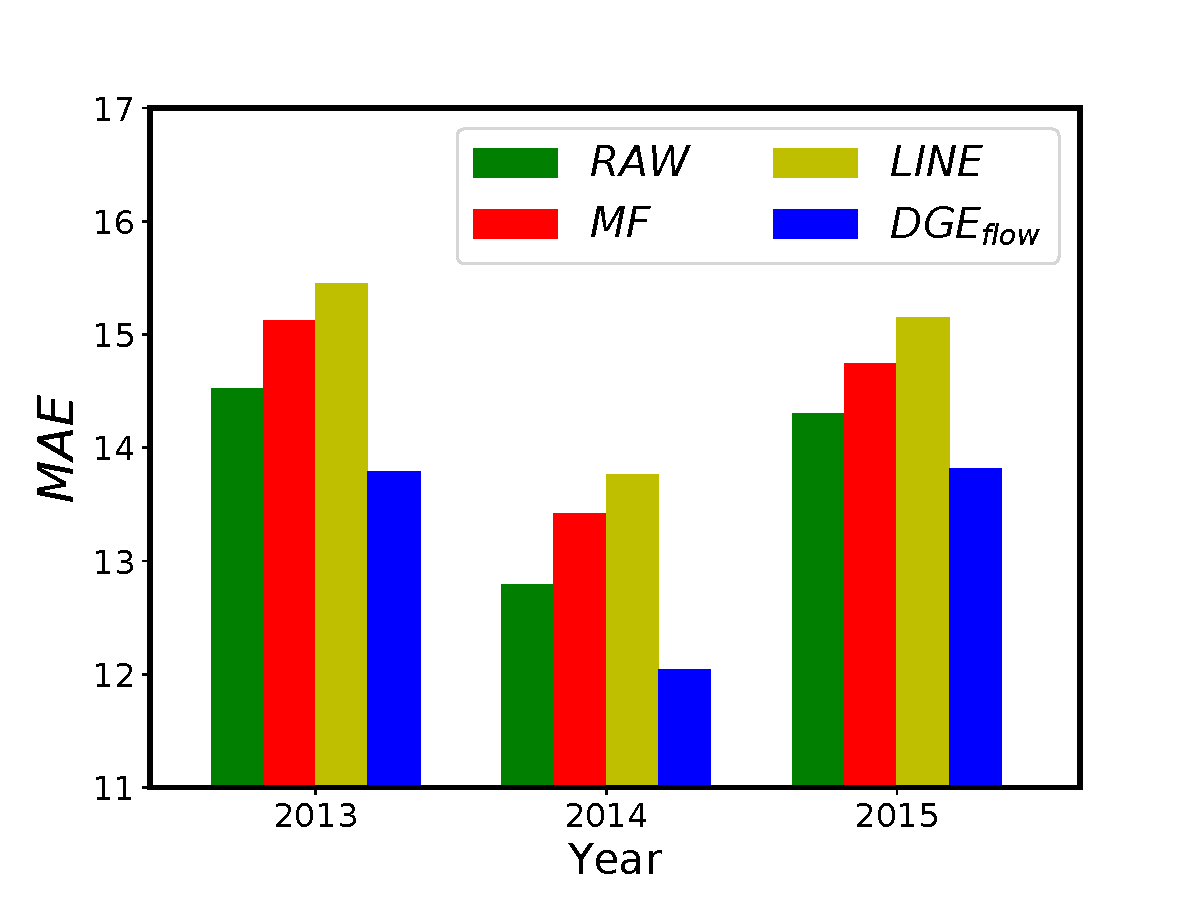
\includegraphics[width=0.48\linewidth]{fig/crime-mae.pdf}
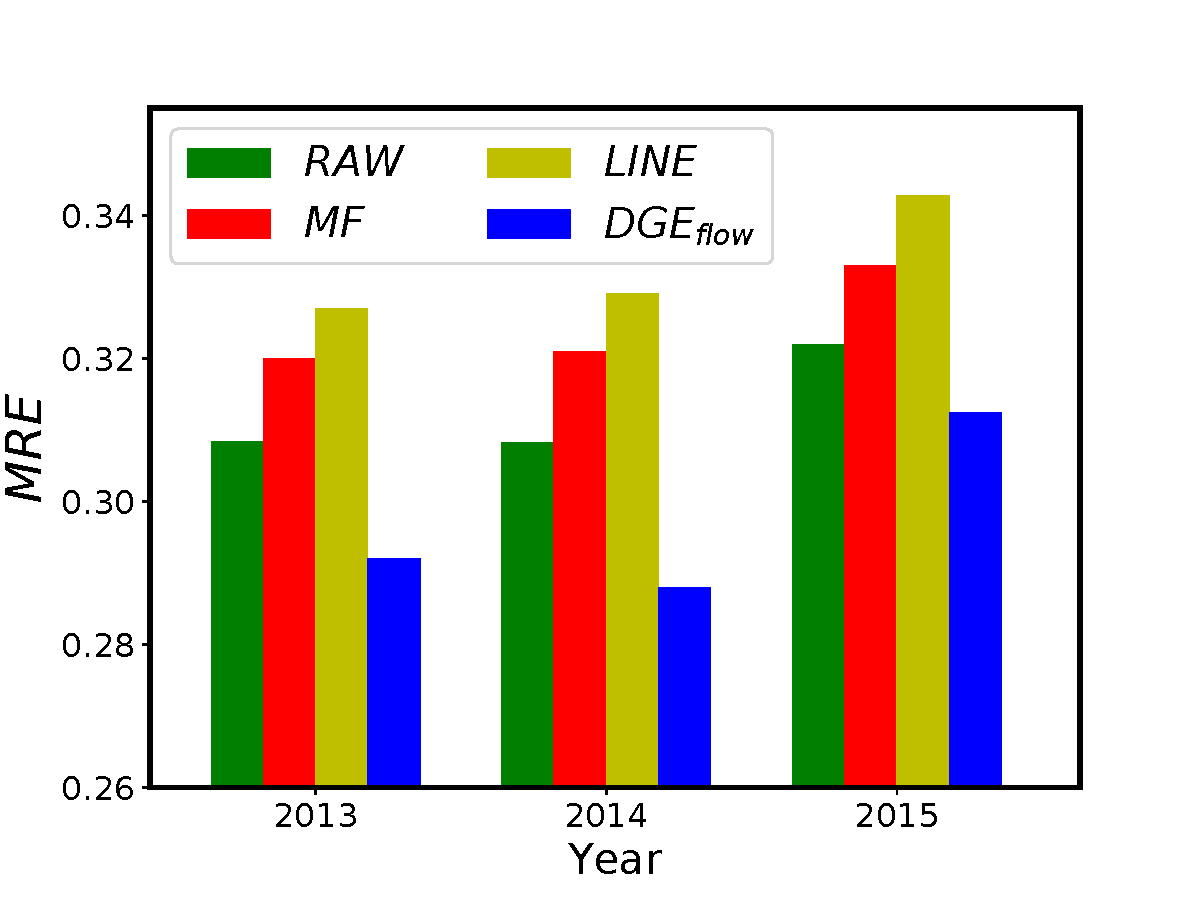
\includegraphics[width=0.48\linewidth]{fig/crime-mre.pdf}
\caption{Crime rate prediction MAE (left) and MRE (right) with dynamic mobility flow embeddings.}
\label{fig:crime}
\end{figure}


The $MAE$ and $MRE$ of crime rate prediction in different years are shown in Figure~\ref{fig:crime}. All methods use D+P+T feature combinations, and the MRE of $RAW$ (green bar) is from the highlighted row in Table~\ref{exp:crime}.

We could see that \dgef consistently has the best performance.  There are two reasons that \dgef is able to outperform $RAW$. First,  \dgef employs the multi-hop structural information, which potentially enables the crime to be propagated for more than one hop. Second, \dgef captures the temporal transition information as well.  $LINE$ and $MF$ have worse performance than \dgef, mainly because embeddings are learned on the independent slotted graph, which does not account for the temporal transition information.



\begin{table}[h]
\centering
\caption{Average personal income and house price prediction with embedding methods.}
\label{tab:other}
\begin{tabular}{|l|r|r|r|r|}
\hline
Data & \multicolumn{2}{c|}{Income} & \multicolumn{2}{c|}{House Price}  \\ \hline
Features & \multicolumn{2}{c|}{D+P+G+T} & \multicolumn{2}{c|}{D+P+T} \\ \hline
Method & MAE & MRE & MAE & MRE  \\ \hline
$RAW$  & 	15127 &  0.250  &  39.28 & 0.229  \\ \hline
$MF$	 &16674  &	0.2756 &	39.83	 &0.233 \\ \hline
$LINE$	 &15534	 &0.2567	 &40.438	 &0.236 \\ \hline
\rowcolor{Gray}
\dgef	 & -	 & -	 &38.95	 &0.226 \\ \hline
\rowcolor{Gray}
\hdge  &14740	 &0.2436 & -  & - \\ \hline
\end{tabular}
\end{table}

We show the embedding methods comparison of average income and house price prediction in Table~\ref{tab:other}. The income prediction uses the feature combination D+P+G+T, while the house price prediction uses the feature combination D+P+T. Similarly, we observe that the proposed \hdge and \dgef are able to learn a better relevance scores respectively, and thus improve the $RAW$ method. The other embedding methods $MF$ and $LINE$, however, lead to a worse performance. This verifies that the proposed flow graph design is necessary to account for the relevance among regions.


\subsubsection{Running Time}
\label{sec:runtime}

We validate the performance gain of applying alias method for random walk sampling on weighted graphs.

\begin{figure}[h]
\centering
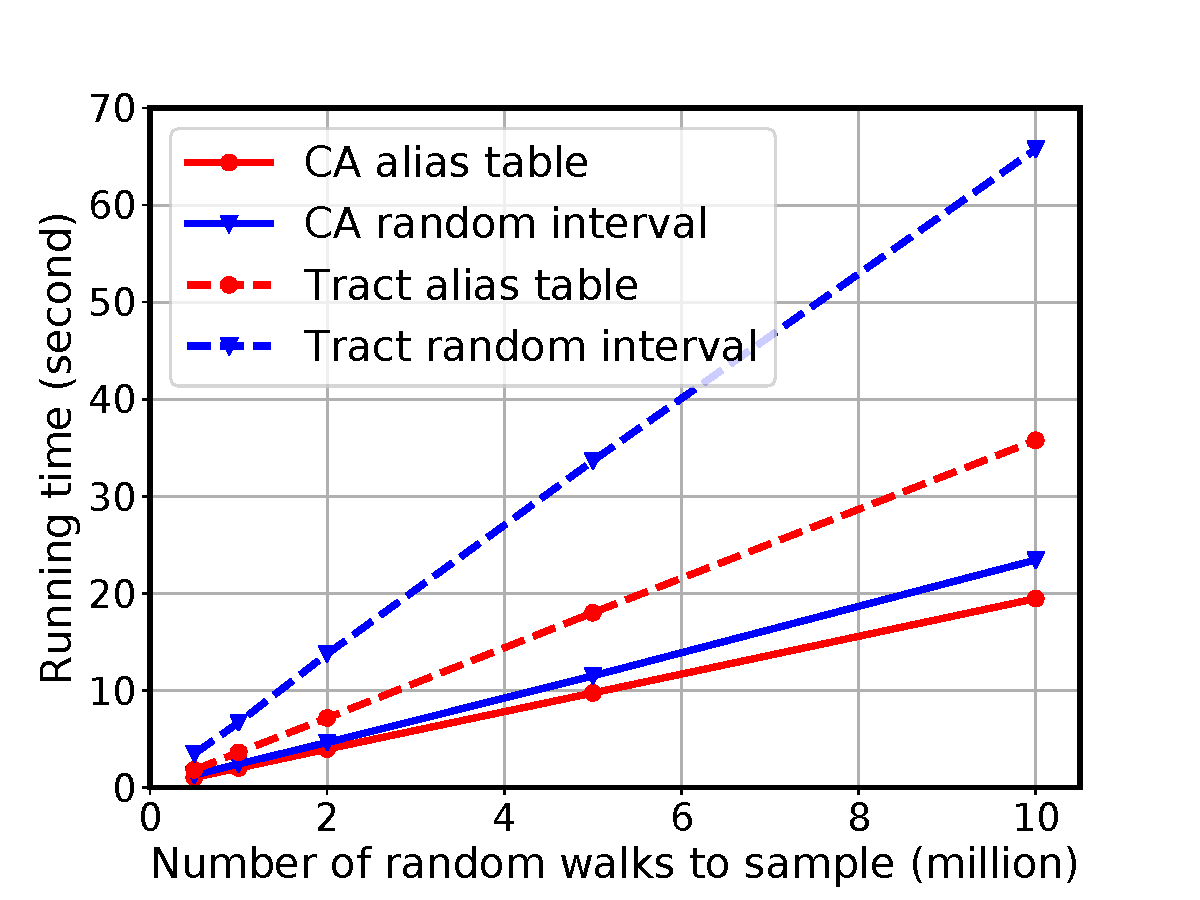
\includegraphics[width=0.6\linewidth]{fig/running-time.pdf}
\caption{The running time of random walk sampling on weighted graphs.}
\label{fig:run}
\end{figure}

In order to validate the efficiency of alias method, we conduct random walk sampling on two flow graphs. The first flow graph is generated at community area level, while the second flow graph is generated at tract level. The tract is a smaller administrative boundary used for the census survey. There are $801$ tracts in Chicago, compared to 77 communities areas. The length of random walks for both graph are bounded by 24. The number of sampled random walks ranges from $500$k to $10$ million.

The running time is shown in Figure~\ref{fig:run}. The compared method is called random interval, which is described in Section~\ref{sec:sample}. It is clear that the alias method consistently runs faster than the random interval method. The alias table method has better performance gain when the number of sampled random walks is large, comparing the solid blue line and solid red line. The reason is that the alias method has a fixed overhead to calculate the alias table for each vertex. Also, the performance gain of alias method on a large graph is bigger. The reason is that alias method reduce the next-vertex sampling complexity from $O(K)$ of the random interval method to $O(1)$, and a larger graph usually has larger $K$, and thus a larger performance gain. 




\subsection{Interpretations}

In this section we give semantic interpretation of the learned dynamic graph embedding. First, we show that \hdge to some degree account for the POI similarity among regions. Next, we use a case study to intuitively explain the semantics captured by \hdge.



\subsubsection{\hdge and POI}

The POI data reflect different functions of urban areas~\cite{yuan2012discovering}, which is a candidate measure of similarity among regions. Our hypothesis is that to certain degree the \hdge accounts for the POI similarity among regions, even though the \hdge learning process does not involve any POI data at all. 

Due to lack of ground truth, we conduct an unsupervised information retrieval experiment to compare different embedding methods. Each region is used as a query, and the goal is to rank other regions according to their similarities to the query region. The POI similarity ranking is used as the ground truth. The quality of various embedding methods are evaluated with the $nDCG$ measures of corresponding rankings.

We use normalized discounted cumulative gain (nDCG) as evaluation measure. Formally, the discounted cumulative gain (DCG) is defined as $DCG@k = \sum_{i=1}^k\frac{rel_i}{\log_2 (i+1)}$, where the relevance $rel_i$ is derived from POI similarity. The nDCG is the DCG normalized by the idea DCG (iDCG), i.e. $nDCG@k = \frac{DCG@k}{iDCG@k}$, 
where $iDCG$ is the DCG of the best ranking. Higher $nDCG@k$ value means better quality of the mobility flow embedding similarity.


We conduct this experiment at tract level, and there are 801 tracts in Chicago. We set the embedding dimension as $20$ for all methods, and divide one day into $8$ 3-hour time slots. To make fair comparison, we sample a subset of tracts that all methods are able to learn embeddings, which results in a set of $419$ tracts.

\begin{figure}[h]
\centering
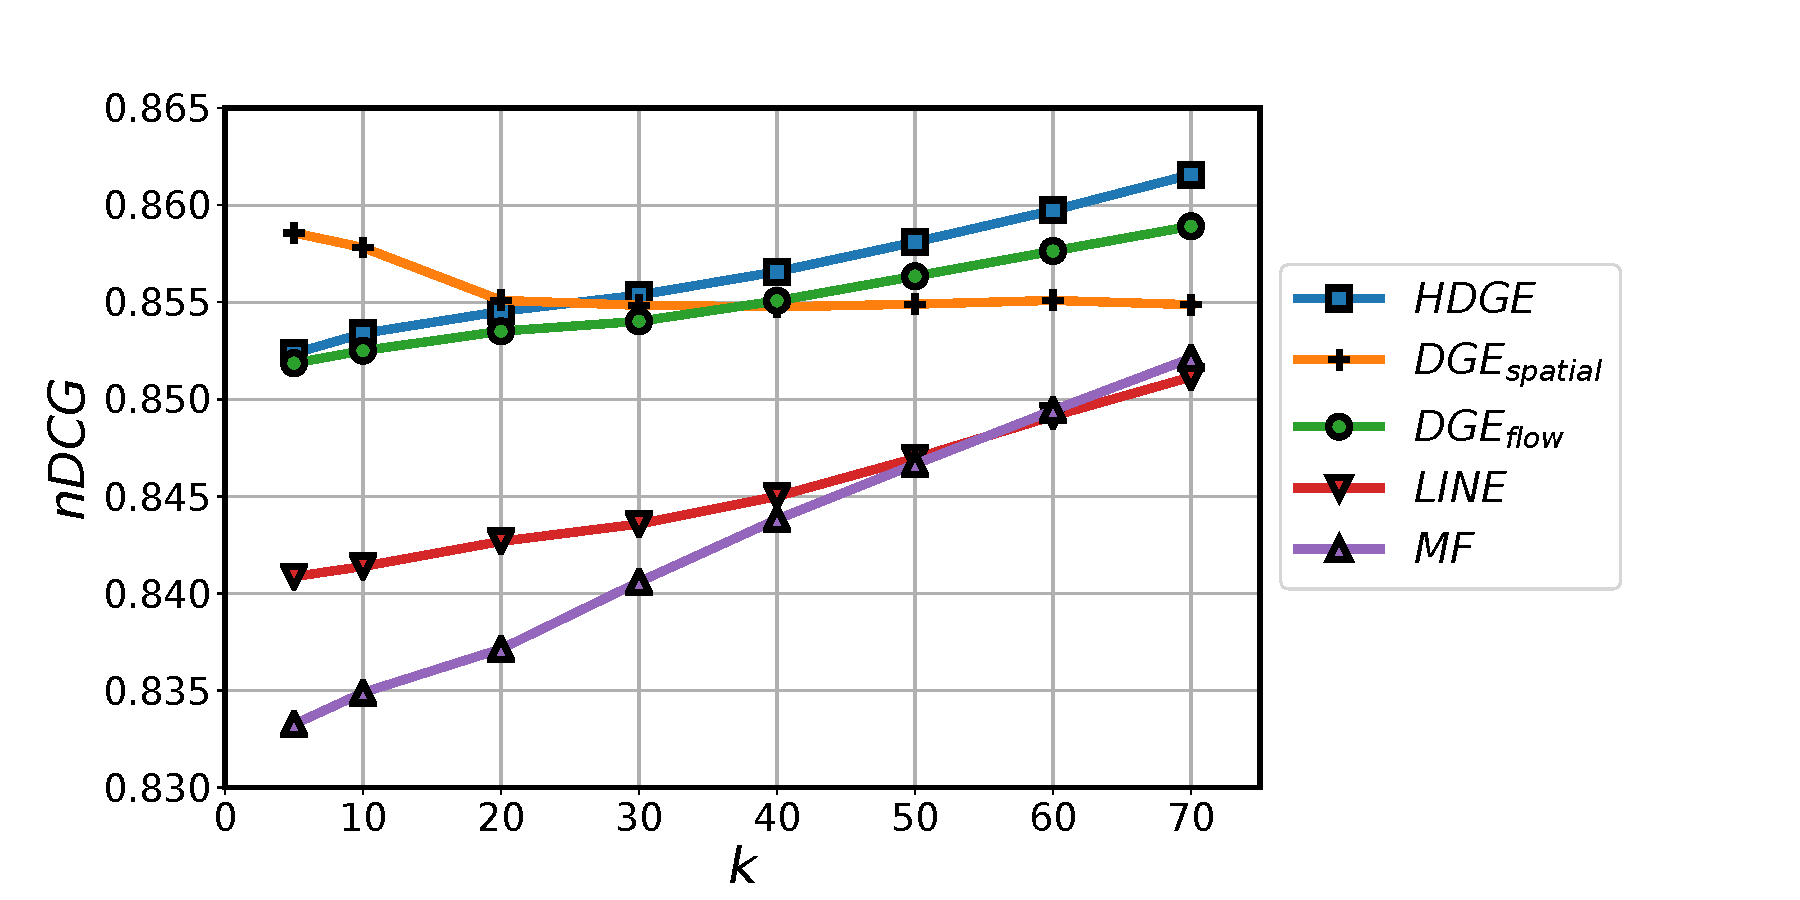
\includegraphics[width=0.8\linewidth]{fig/pairwise-similarity.pdf}
\caption{The $nDCG@k$ plot for various methods with the pairwise similarity evaluation. $k$ is the number of regions to retrieve.}
\label{fig:pairwise-eval}
\end{figure}

\begin{figure*}[t]
\centering
\subfigure[The positions of selected community areas.\label{fig:case-pos}]{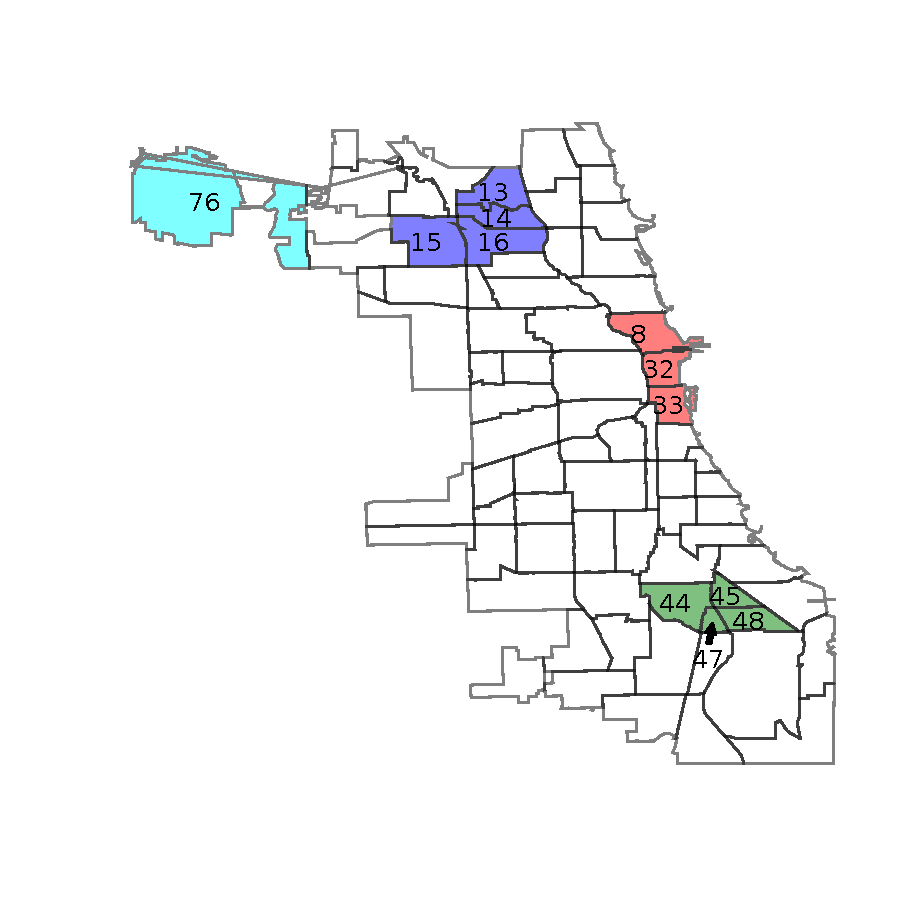
\includegraphics[width=0.32\linewidth]{fig/case-region-on-map.pdf}}
\subfigure[The 2D embedding visualization of selected community areas during different hours.\label{fig:case-2d}]{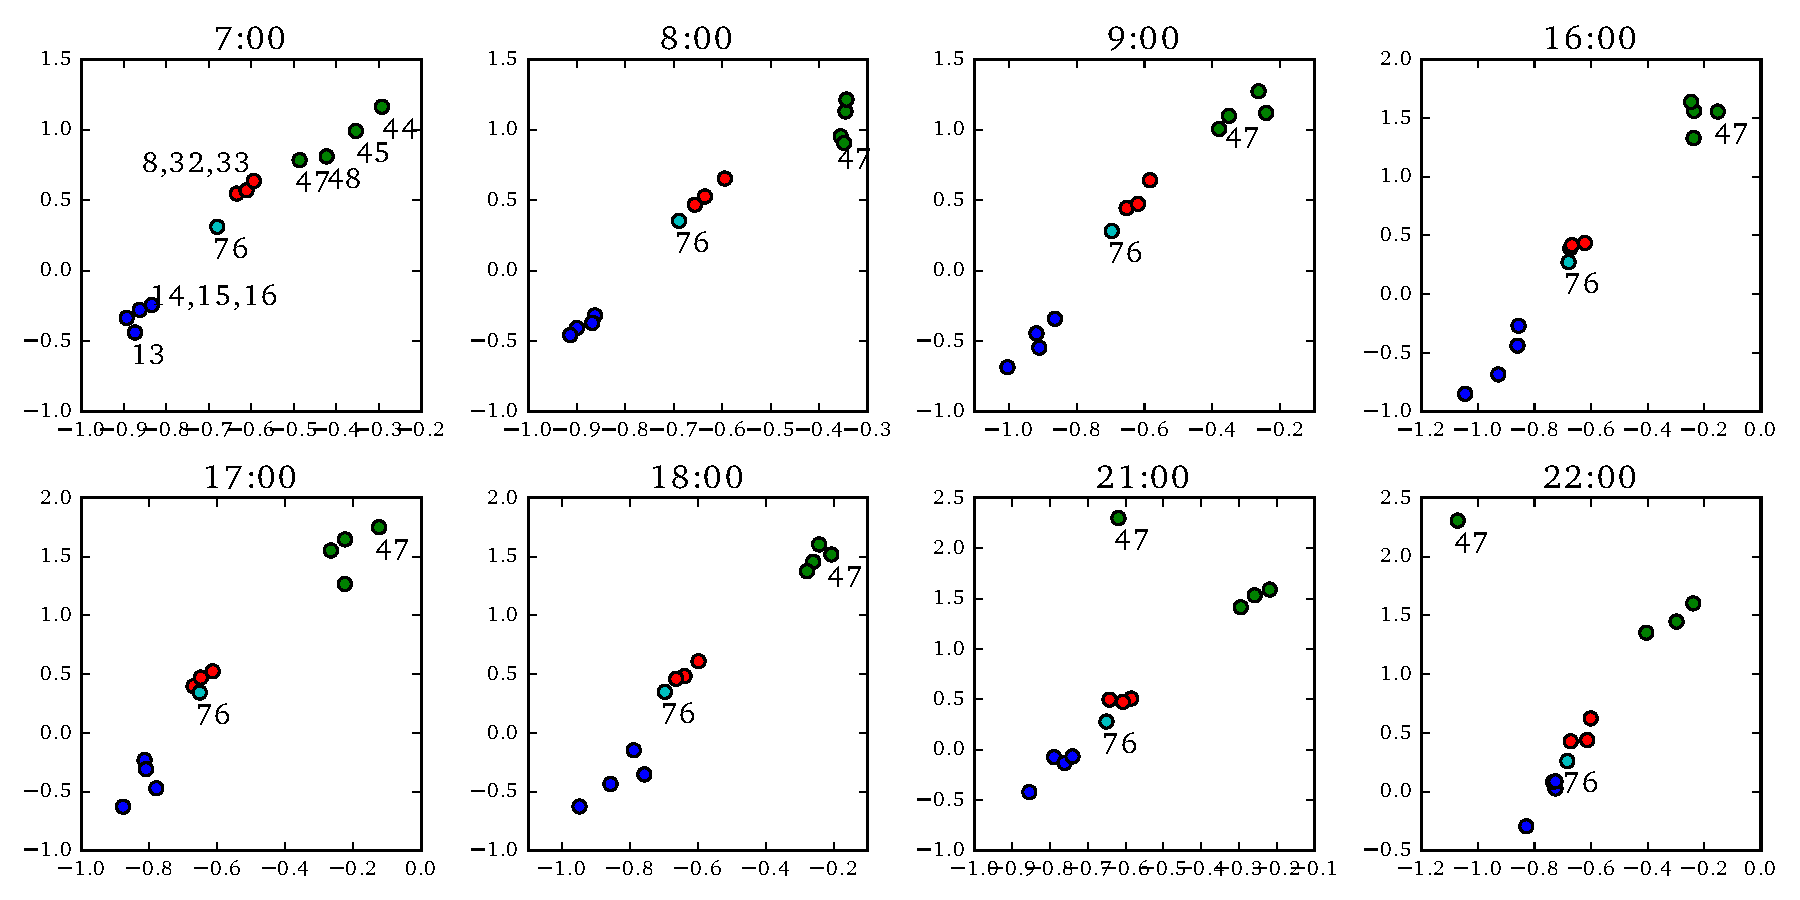
\includegraphics[width=0.65\linewidth]{fig/CA-case-3region.pdf}}
\caption{Case study with 2D visualization. We pick 12 communities areas, whose positions in the city  are shown in (a). The 2D embeddings from different time are visualized in (b). The 12 communities fall in 4 groups: downtown (red), airport (cyan), residential areas (blue), and residential areas with socio-economic issues (green).}
\label{fig:case-study}
\end{figure*}


For each embedding method, we report the average $nDCG@k$ across all tracts over all timestamps. The results are shown in Figure~\ref{fig:pairwise-eval}. From the results we made the following several observations.

Overall, the \hdge method significantly outperform other embedding methods, such as $MF$ and $LINE$. This verifies that the design of flow graph accounts for the POI similarity better than the other embedding methods. The reason is that our flow graph not only consider the temporal dynamics, but also draws connection across different timestamps, which is missing in the slotted graph.




It is interesting to notice that when $k$ is small, the \dges gives the best performance, and the performance decreases as the $k$ increases. The reason is that spatially adjacent tracts usually share similar POI distributions. Therefore, given a query tract, a spatial-based method could easily find adjacent tracts as the results for the top $5$ other tracts that has the most similar POIs. However, when $k$ is larger than $5$, the spatial distance based search does not dominate the results anymore, and thus the performance of \dges decreases.


Although we cannot draw conclusion that \hdge is positively correlate with POI information. This experiment concludes that \hdge design is better than other embedding methods.








\subsubsection{Case Study}


To intuitively demonstrate the semantics of \hdge, we learn a 2-dimensional embedding with \hdge method, and visualize 12 hand-picked community areas that represent four different types of areas.

The locations of these 12 community areas are shown in Figure~\ref{fig:case-pos}. In Figure~\ref{fig:case-pos}, the blue CA 13, 14, 15, and 16 in the north side are densely populated residential areas of the city, where the resident demographics are mostly middle and upper-class. The red CA 8, 32, and 33 locate in downtown, with many commercial, cultural, and financial institutes. In the south of Chicago, the green CA 44, 45, 47 and 48 have different population demographics from the north side. We also plot the Chicago airport, i.e. CA 76, as cyan region. As shown in the map, the Chicago airport locates in the far northwest side of the city, however, it is noteworthy that there are a significant amount of taxi flow commuting between airports and the rest of the city.


In Figure~\ref{fig:case-2d}, we visualize the 2-dimensional embedding of these selected regions from different hours. Particularly, we pick three hours in the morning traffic peak, three hours in the afternoon peak, and two hours at night. 

As expected, we observe that spatially adjacent community areas are close in the \hdge embedding space. Also, mobility flow helps to identify similar regions beyond spatial adjacency, which explains why the CA 76 is close to downtown area.



An interesting case is observed on CA 47. From the visualization we notice that region 47 has a dramatic change from day to night. During the day time, CA 47 is close to its geographical neighbors, i.e. 44, 45, 48, while at night the embedding of CA 47 is far away from most of the communities. After looking into the taxi trips, we found that there is almost no traffic trip going in or out of CA 47 at night. And the reason behind the extremely low taxi volume is that CA 47 suffers from serious gang violence, so that people are trying to avoid this area at night. In Table~\ref{tab:trip-count}, we show the taxi flow and crime rate of CA 47 compared to its neighbors.




\begin{table}[h]
\centering
\caption{CA 47 suffers from serious gang-related violence, and thus has much less traffic flows compared to its neighbors. The total number of taxi in/out trips are in 2013. The crime rate is gang-related crime count per 10,000 population in 2013.}
\label{tab:trip-count}
\begin{tabular}{|c|r|r|r|r|}
\hline
CA & In & Out & Crime rate & Crime rank\\ \hline
44 & 4099 & 5300 & 124 & 7\\ \hline
45 & 857 & 1611 & 112 & 9\\ \hline
\textbf{47} & \textbf{221} & \textbf{287} & \textbf{185} & \textbf{1}\\ \hline
48 & 1935 & 2848 & 72 & 26 \\ \hline
\end{tabular}
\end{table}





% \subsection{Efficiency Study}

% \todo{Influence of number of random sequence on embedding performance}
